\documentclass[12pt,a4paper]{report}

\usepackage[top=3cm,bottom=3cm,left=3cm,right=3cm]{geometry}
%% Packages
%% ========

%% LaTeX Font encoding -- DO NOT CHANGE
\usepackage[OT1]{fontenc}

%% Babel provides support for languages.  'english' uses British
%% English hyphenation and text snippets like "Figure" and
%% "Theorem". Use the option 'ngerman' if your document is in German.
%% Use 'american' for American English.  Note that if you change this,
%% the next LaTeX run may show spurious errors.  Simply run it again.
%% If they persist, remove the .aux file and try again.
\usepackage[english]{babel}

%% Input encoding 'utf8'. In some cases you might need 'utf8x' for
%% extra symbols. Not all editors, especially on Windows, are UTF-8
%% capable, so you may want to use 'latin1' instead.
\usepackage[utf8]{inputenc}

%% This changes default fonts for both text and math mode to use Herman Zapfs
%% excellent Palatino font.  Do not change this.
%\usepackage[sc]{mathpazo}

%% The AMS-LaTeX extensions for mathematical typesetting.  Do not
%% remove.
\usepackage{amsmath,amssymb,amsfonts,amsthm,mathrsfs}

\usepackage[dvipsnames]{xcolor}
\usepackage{tcolorbox}

%% LaTeX' own graphics handling
\usepackage{graphicx}

%% This allows you to add .pdf files. It is used to add the
%% declaration of originality.
\usepackage{pdfpages}

\usepackage{mathtools}

\numberwithin{equation}{section}

\newtheoremstyle{mystyle}% ⟨name ⟩ 
{3pt}% ⟨Space above ⟩1 
{3pt}% ⟨Space below ⟩1
{}% ⟨Body font ⟩
{}% ⟨Indent amount ⟩2
{\sffamily}% ⟨Theorem head font⟩
{.}% ⟨Punctuation after theorem head ⟩
{.5em}% ⟨Space after theorem head ⟩3
{}% ⟨Theorem head spec (can be left empty, meaning ‘normal’)⟩
%
%
%\newtheoremstyle{break}%
%{}{}%
%{}{}%
%{\bfseries}{}%  % Note that final punctuation is omitted.
%{\newline}{}

\theoremstyle{mystyle}

\newtheorem{definition}{Definition}[section]
\newtheorem{theorem}[definition]{Theorem}
\newtheorem{lemma}[definition]{Lemma}
\newtheorem{corollary}[definition]{Corollary}
\newtheorem{proposition}[definition]{Proposition}
\newtheorem{example}[definition]{Example}
%\tcbuselibrary{theorems}
\tcbuselibrary{skins,breakable}



\tcolorboxenvironment{theorem}{
	enhanced jigsaw,colframe=Salmon!90!Black,interior hidden, breakable,before skip=10pt,after skip=10pt 
}

\tcolorboxenvironment{proposition}{
	blanker,breakable,left=5mm,
	before skip=10pt,after skip=10pt,
	borderline west={1mm}{0pt}{Green!70}
}

\tcolorboxenvironment{definition}{
	blanker,breakable,left=5mm,
	before skip=10pt,after skip=10pt,
	borderline west={1mm}{0pt}{cyan!40!black}
}

\tcolorboxenvironment{example}{
	blanker,breakable,left=5mm,
	before skip=10pt,after skip=10pt,
	borderline west={1mm}{0pt}{green!35!black}
}

\tcolorboxenvironment{lemma}{
	blanker,breakable,left=5mm,
	before skip=10pt,after skip=10pt,
	borderline west={1mm}{0pt}{RoyalPurple!55!Aquamarine!100!}
}

\tcolorboxenvironment{corollary}{
	blanker,breakable,left=5mm,
	before skip=10pt,after skip=10pt,
	borderline west={1mm}{0pt}{CornflowerBlue!60!Black}
}




\tcolorboxenvironment{proof}{% `proof' from `amsthm' 
	blanker,breakable,right=5mm,
	before skip=10pt,after skip=10pt,
	borderline east={0.5mm}{1pt}{red!10!white}}

\usepackage[linkcolor=blue,colorlinks=cyan,citecolor=red,filecolor=black]{hyperref}

\usepackage{hyperref}
\hypersetup{
	colorlinks = true,
	linkcolor=NavyBlue,
	citecolor=Orange,
	filecolor=orange}

\usepackage{tikz}
\usetikzlibrary{calc}
\usetikzlibrary{cd}


\newcommand{\R}{\mathbb{R}}
\newcommand{\C}{\mathbb{C}}
\newcommand{\Z}{\mathbb{Z}}
\newcommand{\N}{\mathbb{N}}
\newcommand{\K}{\mathbb{K}}
\renewcommand{\d}{\mathrm{d}}
\renewcommand{\i}{\mathbf{\mathrm{i}}}


\newcommand{\abs}[1]{\left\lvert #1 \right\rvert}
\newcommand{\norm}[1]{\left\lVert #1 \right\rVert}
\newcommand{\inner}[1]{\left\langle #1 \right\rangle}

\newcommand{\clin}{\operatorname{clin}}
\newcommand{\spn}{\operatorname{span}}
\newcommand{\dist}{\operatorname{dist}}
\newcommand{\range}{\operatorname{range}}

\let\oldemptyset\emptyset
\let\emptyset\varnothing


\title{Notes on Measure and Probability Theory}
\author{Liu Zhizhou}
\date{First Created: September 6, 2022\\
	Last Modified: \today}



\begin{document}
	{\sffamily \maketitle}
	
	
	\tableofcontents

	
	\newcommand{\A}{\mathscr{A}}
	\part{Measure Theory}
	\section{An Introduction: From Riemann Integral to Measure Theory}
	\paragraph{Riemann Integral}
	A viewpoint of understanding Riemann Integral is considering the upper sum and lower sum, namely
	$$
	U_p(R,f)\triangleq \sum_{j=1}^n (x_j-x_{j-1})M_i,
	\quad 
	L_p(R,f)\triangleq \sum_{j=1}^n (x_j-x_{j-1})m_i,
	$$
	where $M_i=\sup_{x\in [x_{j-1},x_j]}f(x)$, $m_i=\inf_{x\in [x_{j-1},x_j]}f(x)$, $p$ is the partition and $R$ means we are in the case of Riemann.
	Then define
	$$
	\overline{\int_a^b} f(x) \d x\triangleq\inf_p U_p(R,f),
	\quad
	\underline{\int_a^b} f(x) \d x\triangleq\sup_p L_p(R,f).
	$$
	If the two values above equal, then we say the $f(x)$ is Riemann integrable. There are two import results in Riemann integral.
	\begin{proposition}
		Every continuous real-valued function on each closed bounded interval is Riemann integrable.
	\end{proposition}
	And also the following theorem.
	\begin{theorem}
		Let $(f_n)_{n=1}^\infty$ a sequence of Riemann integrable functions on $[a,b]$. Suppose that it converges uniformly on $[a,b]$ to a function $f$. Then $f$ is Riemann integrable.
	\end{theorem}
	This two results seems nice and make the integral apply to different areas. However, there are issues that occur in Riemann integral.
	\begin{enumerate}
		\item Many ``simple'' functions are not Riemann integrable. For example, the Dirichlet function defined below.
		$$
		D(x)\triangleq \begin{cases}
			1, &x\in \mathbb{Q}\\
			0, &x\notin \mathbb{Q}
		\end{cases}.
		$$
		It is not Riemann integrable since the upper integral equals $b-a$ yet the lower integral equals zero.
		\item If $0\leq f_1\leq f_2\leq \dots$ and $f_i$ is Riemann integrable for each $i\in \N$. The pointwise convergent of $f_n\to f$ does not grantee that $f$ is Riemann integrable. Indeed, let $\mathbb{Q}=\{r_1,r_2,\dots\}$. Define
		$$
		f_n(x)=
		\begin{cases}
			1, & x\in \{r_1,\dots,r_n\}\\
			0, & x\notin \{r_1,\dots,r_n\}
		\end{cases}.
		$$
		Then for each $x$, $f_n(x)\to D(x)$. Note that $f_n$ is Riemann integrable for each $n$.
		\item Suppose $f_n\geq 0$ for all $n$ and Riemann integrable. The equation
		\begin{equation}
			\int_a^b \sum_{i=1}^\infty f_n(x)= \sum_{n=1}^\infty \int_a^b f_n(x)
		\end{equation}
		is not true in general. Consider
		$$
		f_n(x)=
		\begin{cases}
			1, & x=r_n\\
			0, & x\neq r_n
		\end{cases}.
		$$
		Then $\sum_{i=1}^\infty f_n(x)=D(x)$. The right hand side of the equation is even not integrable.
	\end{enumerate}
	Here comes Lebesgue who defined Lebesgue Integral to fix the above problems.
	
	\paragraph{Lebesgue Integral}
		\begin{figure}
		\centering
		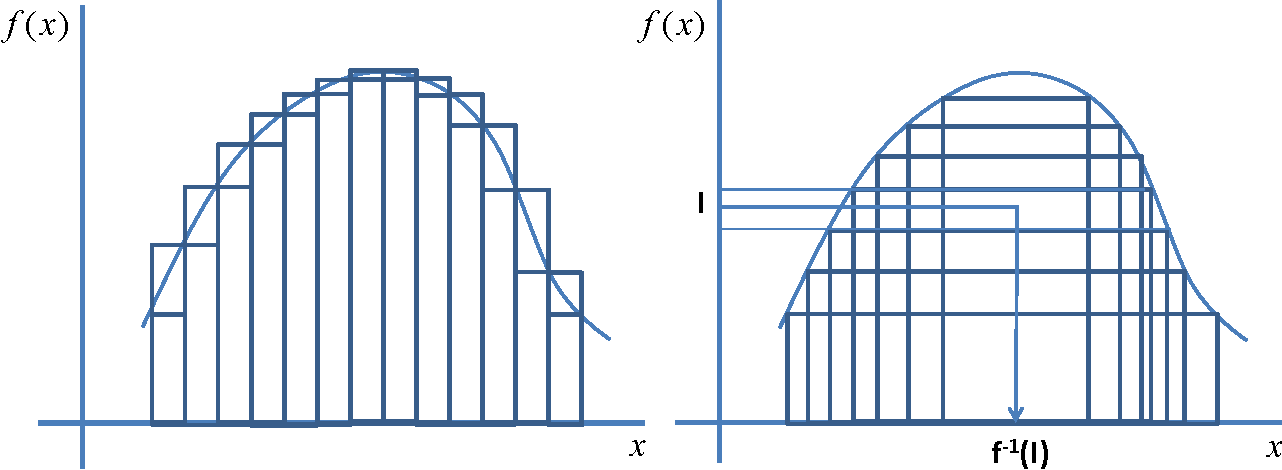
\includegraphics[width=0.80\textwidth]{figures/Riem-Leb.jpg}
		\caption{The figure one the left is an illustration of Riemann Integral; on the right is an illustration of Lebesgue Integral.}
	\end{figure}
	
	Consider an easy case: the domain of $f$ is $[a,b]$. Rather than considering the partition on $[a,b]$ as in Riemann Integral, Lebesgue considered the partial on the range of $f$. The preimage would then be
	$$
	E_i=\{x: y_{i-1}<f(x_i)\leq y_i\}.
	$$
	The corresponding upper sum and lower sum is
	$$
	U_p(L,f)\triangleq\sum_{i=1}^n y_i l(E_i),
	\quad
	L_p(L,f)\triangleq\sum_{i=1}^n y_{i-1} l(E_i),
	$$
	where $l(E_i)$ is the length of $E_i$. Then
	\begin{equation}\label{eq:Lebesgue difference}
		U_p(L,f)-L_p(L,f)=\sum_{i=1}^n (y_i-y_{i-1})l(E_i)\leq \max_i\{y_i-y_{i-1}\}(b-a).
	\end{equation}
	Therefore, $U_p(L,f)=L_p(L,f)$ when $\max_i\{y_i-y_{i-1}\}\to 0$. It seems that the integral is well-defined already and all functions are ``Lebesgue Integrable''. However, the issue is: what is $l(E_i)$? How to calculate it?
	
	Since the only knowledge about length is the case of $E_i$ is interval, we have no choice but to do the following definition, which is called \emph{(Lebesgue) outer measure},
	$$
	\mu^* (E)\triangleq \inf\{\sum_{i=1}^\infty |I_i|: E\subset \cup_{i=1}^\infty I_i, \text{ where $I_i$ is open interval}\}.
	$$
	However, this measure does not have the countable additive property when $\{E_i\}$ are disjoint. Instead, it only has sub-additive property:
	$$
	\mu^* (\cup_{i=1}^\infty E_i)\leq \sum_{i=1}^\infty \mu^* (E_i),
	$$
	which does not guarantee Eq. (\ref{eq:Lebesgue difference}) to be true. 
	
	The definition of Lebesgue measure fixed the problem. There are many equivalent definitions of Lebesgue measure:
	\begin{proposition}\label{prop:equivalent definitions of measurable}
		The following definitions are equivalent:
		\begin{enumerate}
			\item Suppose $\mu_*(E)=\sup\{\mu^*(A): A\subseteq E, \text{ where $A$ is closed}\}$, which is called the \emph{(Lebesgue) outer measure} of $E$. If $\mu^*(E)=\mu_*(E)$, then we say that $E$ is measurable.
			\item If for any $\epsilon>0$, there exists an open set $U$ with $E\subset U$ such that $\mu^*(U-E)\leq \epsilon$, then we say that $E$ is measurable.
			\item If for any subset $A$, we have
			\begin{equation}
				\mu^*(A) = \mu^*(A\cap E)+\mu^*(A\cap E^c),
			\end{equation}
			then we say that $E$ is measurable.
		\end{enumerate}
	\end{proposition}
	We can show that for every measurable set, 
	$$
	\mu^* (\cup_{i=1}^\infty E_i)\leq \sum_{i=1}^\infty \mu^* (E_i).
	$$
	Then define \emph{measurable function} to be the functions that satisfies $f^{-1}([-\infty,a])$ is measurable for all $a\in \R$. Then the issue explained after Eq. (\ref{eq:Lebesgue difference}) is completely solved.
	
	
	\paragraph{Measure Theory}
	The result in $\R$ can be easily generalize to the case of $\R^n$, however, how to define measure in abstract spaces, for example,  the $L^2$ space. A Mathematician called Frechet used the same procedure defined the measure in abstract spaces: first define open set, then the measure on those sets, and the outer measure... However, have a second look at the Proposition \ref{prop:equivalent definitions of measurable}, we find that item 3 does not need any information of open sets! Therefore, the definition of measurable set in abstract space follows.
	
	
	
	
	
	
	
	\chapter{Fundamental Concepts}
	\section{Algebra and $\sigma$-algebra}
	\begin{definition}[algebra]
		A non-empty subset $\A\subset 2^X$ is said to be an \emph{algebra} if
		\begin{enumerate}
			\item $\emptyset \in \A$,
			\item if $A\in \A$, then $A^c\in \A$;
			\item if $A_1,\dots,A_n\in \A$, then $\cup_{i=1}^n A_i\in \A$.
		\end{enumerate}
	\end{definition}
	
	\begin{definition}[$\sigma$-algebra]
		A non-empty subset $\A\subset 2^X$ is said to be an \emph{algebra} if
		\begin{enumerate}
			\item $\emptyset \in \A$,
			\item if $A\in \A$, then $A^c\in \A$;
			\item if $A_1,A_2\dots\in \A$, then $\cup_{i=1}^\infty A_i\in \A$.
		\end{enumerate}
	\end{definition}
	In this case, we call $(X,\A)$ a \emph{measurable space} and the elements of $\A$ is called \emph{$\A$-measurable sets} (or simply measurable sets).
	
	Sometimes $\mathscr{C}\subset 2^X$ is not a $\sigma$-algebra.
	\begin{definition}
		Assume $\mathscr{C}\subset 2^X$. The $\sigma$-algebra generated by $\mathscr{C}$ is the smallest $\sigma$-algebra containing $\mathscr{C}$, denoted $\sigma(\mathscr{C})$.
	\end{definition}
	Note that $\sigma(\mathscr{C})$ is all the intersection of all $\sigma$-algebra that contains $\mathscr{C}$.
	
	\begin{definition}[Borel $\sigma$-algebra]
		If $X$ is a topological space, the $\sigma$-algebra generated by all open subsets of $X$ is called the Borel $\sigma$-algebra of $X$ and it is denoted by $\mathscr{B}(X)$.
	\end{definition}
	
	
	
	\renewcommand{\Pr}{\mathbb{P}}
	\part{Probability Theory}
	\chapter{Fundamental Concepts}
	\section{Intuition of Probability}
	We have the following concepts illustrated in words. A \emph{sample space} (or state space), denoted $\Omega$, is the space of all possible outcomes of a \emph{random experiment}, where the random experiment is a kind of experiment that you could not know the outcome before implementing. A \emph{(random) event} is a subset of sample space.
	
	Intuitively, the probability of an event $A$, denoted $\Pr(A)$, is the frequency that $A$ will occur if we repeat the experiment many times, i.e.
	\begin{equation}
		\Pr(A)=\lim_{n\to\infty} f_n(A),
	\end{equation}
	where $f_n(A)$ is the frequency of $A$ after $n$ trials of experiments.
	
	The \emph{probability model} is a triple-set $(\Omega,\A,\Pr)$, where $\A$ is the class of events which we can define probability. For example, if $\Omega=\R$, then $\A$ could be all Lebesgue measurable set or all Borel sets.
	
	A \emph{random variable} $X(\omega)$ is a function which maps $\Omega\to E$, where $E$ is a ``simple'' space, often $\R$ or $\R^n$ and even a Banach space or Hilbert space. And we can induce a probability on $E$ by the probability on $\Omega$. Define for $B\subseteq E$, 
	\begin{equation*}
		X^{-1}(B)=\{\omega\in \Omega:X(\omega)\in B\}
	\end{equation*}
	and
	\begin{equation}
		\Pr_X(B)=\Pr(X^{-1}(B)).
	\end{equation}
	Then we have a new probability model $(E,\mathscr{E},\Pr_X)$. And $\Pr_X$ is called the \emph{distribution} of $X$.



\end{document}